\subsection{Listas y operaciones comunes}
Las listas en python son un conjunto ordenado y editable de elementos, son dinámicas esto quiere decir que puede contener diferente tipos de datos, y aparte cabe recalcar que puede tener elementos duplicados y no generará error. Estas se pueden ocupar tanto como para recopilar datos como para organizar y alguna de sus funciones son las siguientes:

\begin{itemize}
    \item Creación de listas: Se puede crear una listas abriendo corchetes ``[]'' y separando los datos por comas ``,''
    \begin{figure}[h]
        \centering
        \scalebox{0.35}{
        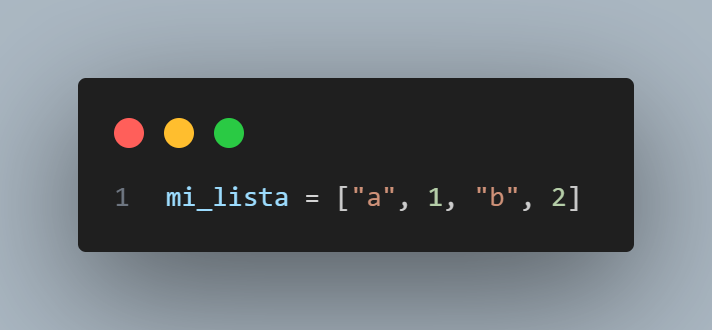
\includegraphics{Imagenes/listas1.png}
        }
      \end{figure}
    \newpage
    \item Acceso a elementos: se puede acceder a un elemento en específico de la lista poniendo el nombre de este y dentro de corchetes el número en el lugar que se encuentra  (se empieza a contar desde el 0, y para seleccionar el último será -1).
    \begin{figure}[h]
        \centering
        \scalebox{0.35}{
        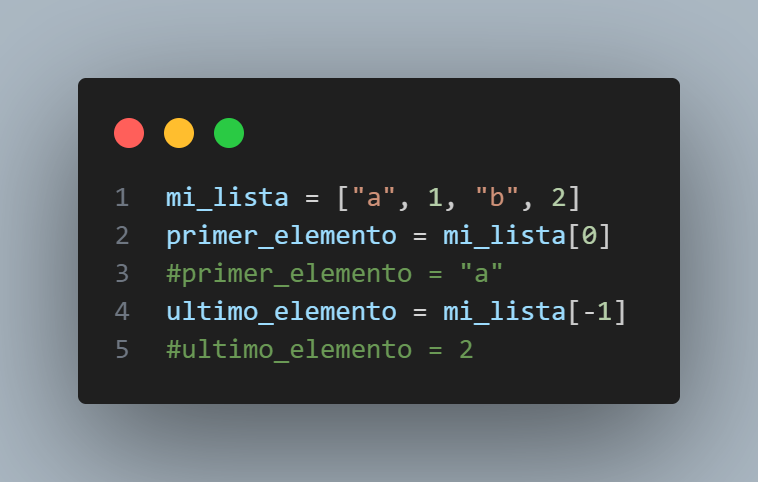
\includegraphics{Imagenes/listas2.png}
        }
      \end{figure}
    
    \item Modificar elementos: Seleccionando el puesto en el que se encuentra el dato e igualarlo al valor que queramos.
    \begin{figure}[h]
        \centering
        \scalebox{0.35}{
        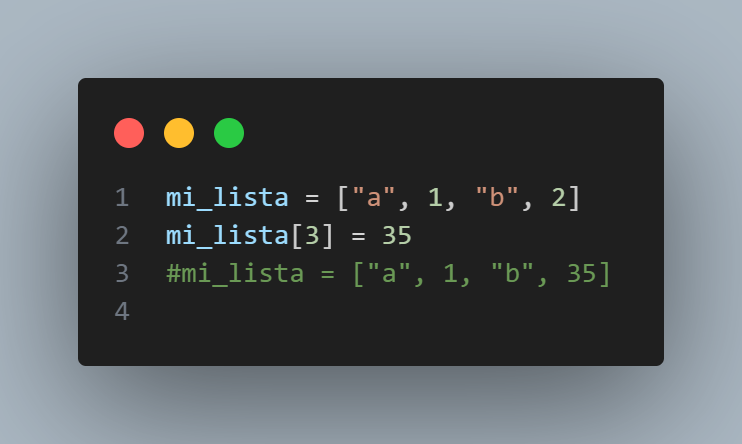
\includegraphics{Imagenes/listas3.png}
        }
      \end{figure}
    \newpage
    \item Añadir elementos: Utilizando el método ``.append(elemento)'' se pueden agregar datos.
    \begin{figure}[h]
        \centering
        \scalebox{0.35}{
        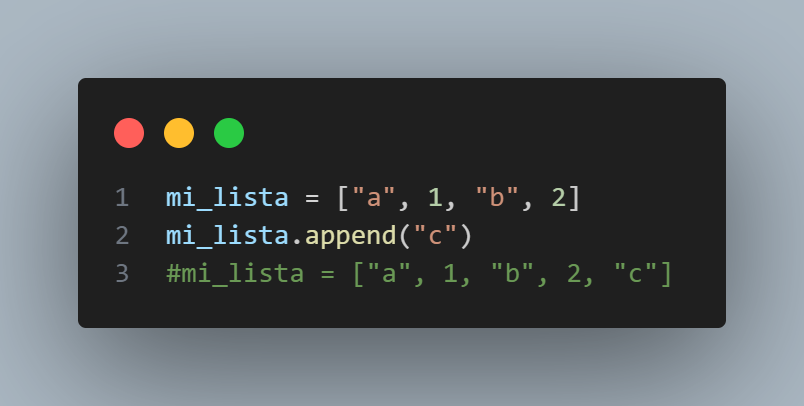
\includegraphics{Imagenes/listas4.png}
        }
      \end{figure}
    
    \item Insertar elementos: Si bien cumple la misma función que se describió anteriormente se ocupa el método ``.insert(posición, elemento)'' con esta también se puede detallar la posición en que queremos que esté.
    \begin{figure}[h]
        \centering
        \scalebox{0.35}{
        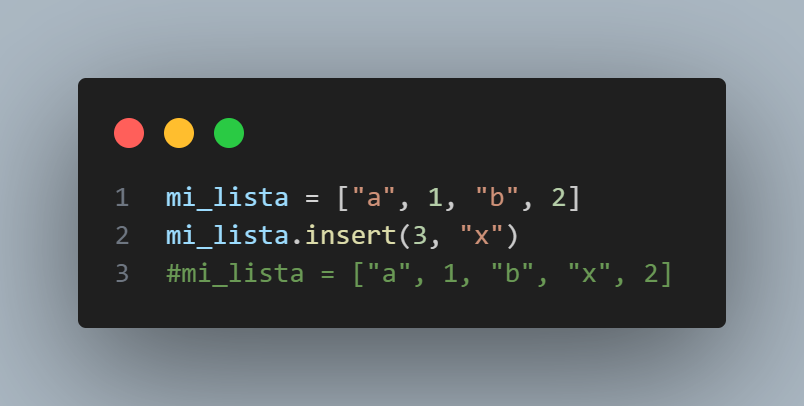
\includegraphics{Imagenes/listas5.png}
        }
      \end{figure}
    
    \item Eliminar elementos: Para eliminar elementos hay dos métodos el ``.pop(lugar del elemento)'' que elimina el dato que haya en ese puesto y el ``.remove(elemento)'' que elimina el elemento que se mencionó en los paréntesis.
    \begin{figure}[h]
        \centering
        \scalebox{0.35}{
        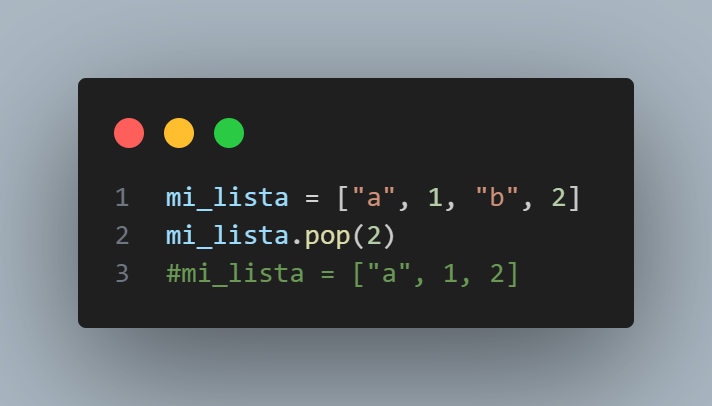
\includegraphics{Imagenes/listas6.png}
        }
      \end{figure}
    
      \begin{figure}[h]
        \centering
        \scalebox{0.35}{
        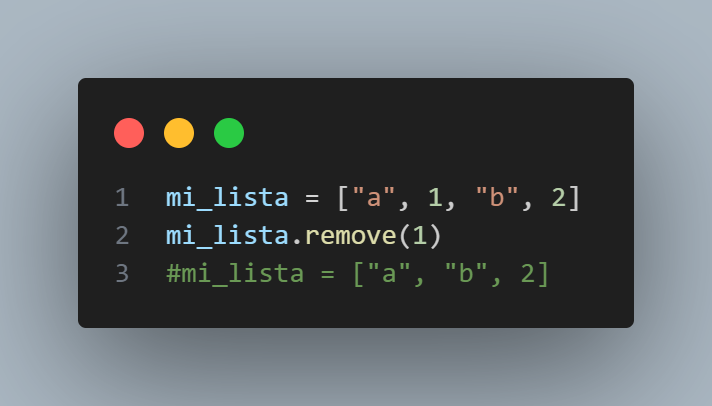
\includegraphics{Imagenes/listas7.png}
        }
      \end{figure}
\newpage
    \item Largo de una lista: Para saber cuántos elementos hay en la lista ocupamos el método ``.len(mi\_lista)''.
    \begin{figure}[h]
        \centering
        \scalebox{0.35}{
        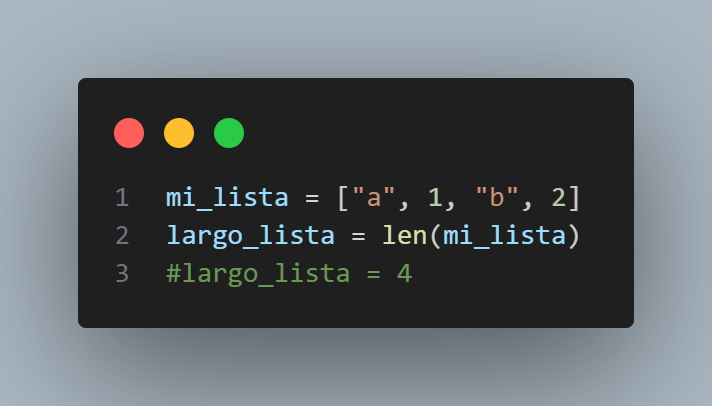
\includegraphics{Imagenes/listas8.png}
        }
      \end{figure}
    
    \item Rebanado(slicing): Puedes acceder a una porción de una lista utilizando el operador de rebanado ``[:]''.
    \begin{figure}[h]
        \centering
        \scalebox{0.35}{
        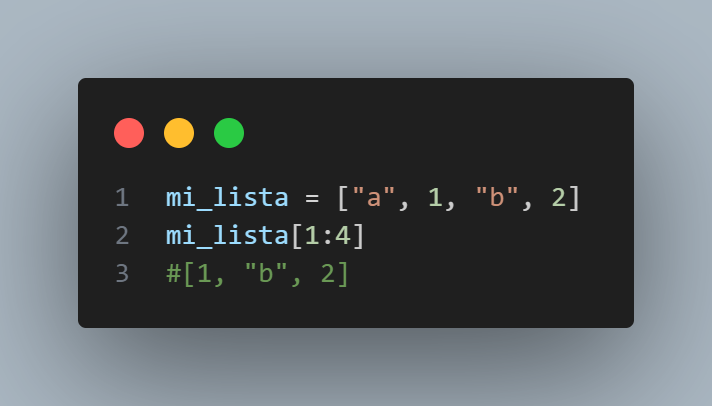
\includegraphics{Imagenes/listas9.png}
        }
      \end{figure}
    \newpage
    \item Concatenación de listas: Se pueden unir dos o más listas utilizando el operador de concatenación ``+''. 
    \begin{figure}[h]
        \centering
        \scalebox{0.35}{
        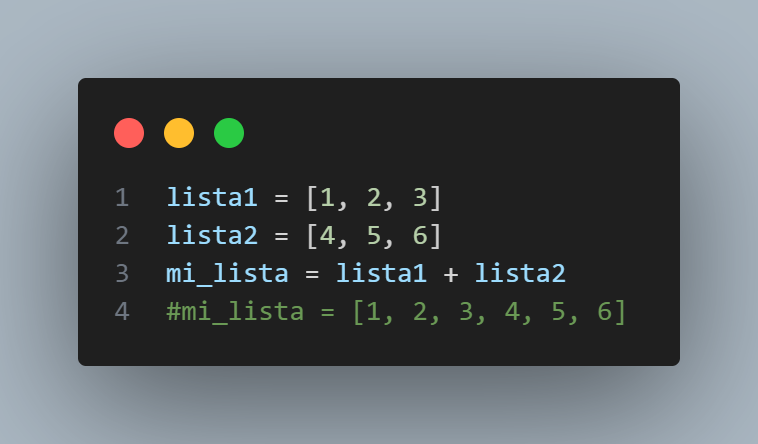
\includegraphics{Imagenes/listas10.png}
        }
      \end{figure}
    
    \item Ordenar una lista: Para ordenar una lista de manera ascendente o descendente se pueden utilizar los métodos ``.sort()'' o ``.sorted()'' respectivamente.
    \begin{figure}[h]
        \centering
        \scalebox{0.35}{
        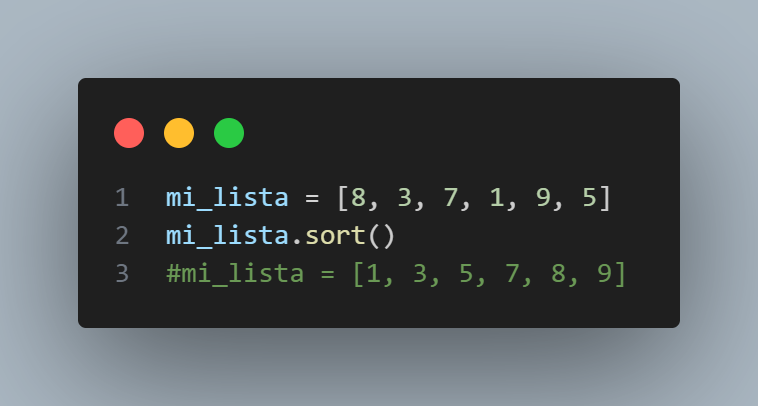
\includegraphics{Imagenes/listas11.png}
        }
      \end{figure}

      \begin{figure}[h]
        \centering
        \scalebox{0.35}{
        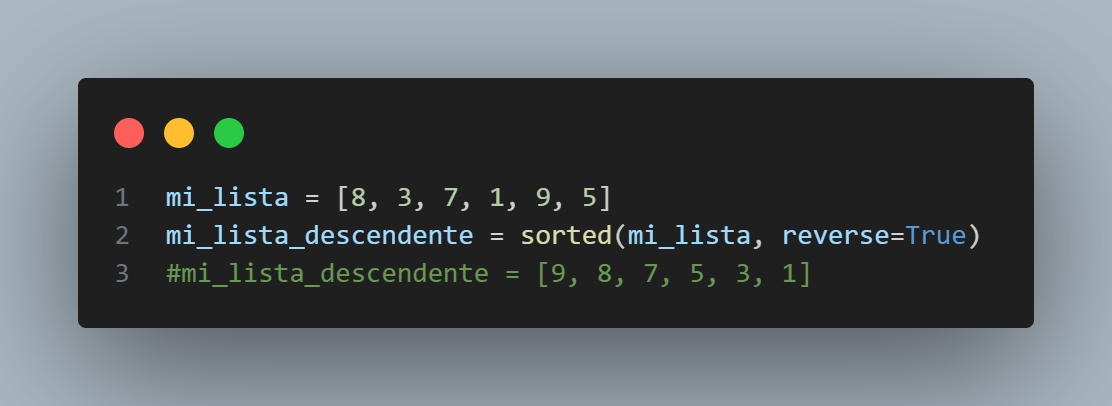
\includegraphics{Imagenes/listas12.png}
        }
      \end{figure}
    \newpage
    \item Buscar elementos:Se puede buscar un elemento de la lista utilizando el operador “in” o el método ``.index(elemento)''.
    \begin{figure}[h]
        \centering
        \scalebox{0.35}{
        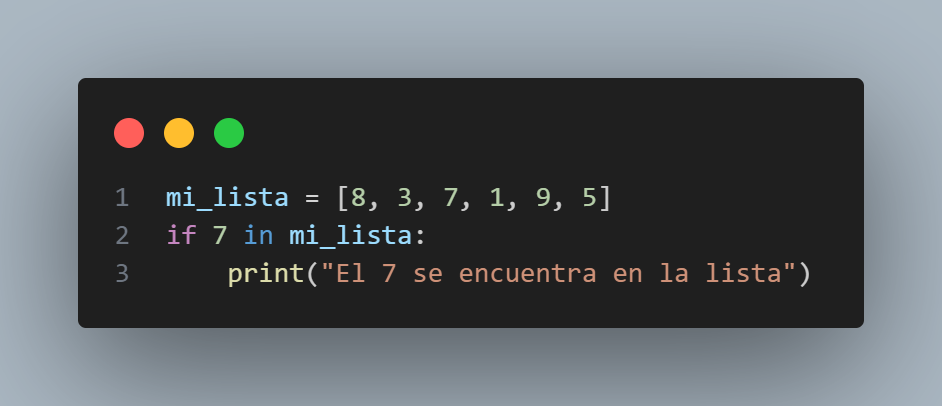
\includegraphics{Imagenes/listas13.png}
        }
      \end{figure}
    
      \begin{figure}[h]
        \centering
        \scalebox{0.35}{
        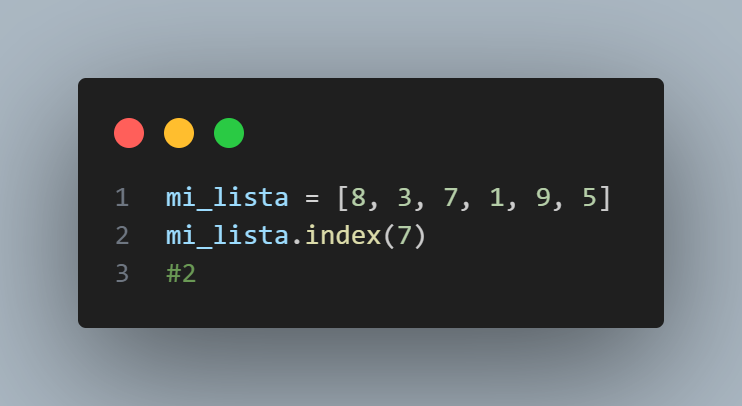
\includegraphics{Imagenes/listas14.png}
        }
      \end{figure}
\end{itemize}

\subsection{Tuplas y sus propiedades}
Si bien las tuplas son un conjunto de datos similares a las listas estas son inmutables esto quiere decir que una vez creada no se puede volver a modificar, algunas de sus propiedades son:

\begin{itemize}
    \item Creación de tuplas: Primero que nada para crear una tupla solo se necesita de paréntesis ``()'' y separar los datos por comas ``,'', aunque también se pueden crear solo separando los elementos con comas.
    \begin{figure}[h]
        \centering
        \scalebox{0.35}{
        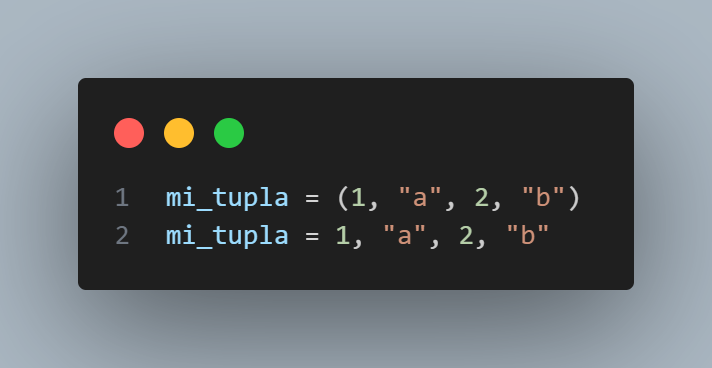
\includegraphics{Imagenes/listas15.png}
        }
      \end{figure}

    \item Acceso a elementos: Al igual que en las listas para acceder a un elemento en especifico solo se necesita de corchetes ``[índice]''.
    \begin{figure}[h]
        \centering
        \scalebox{0.35}{
        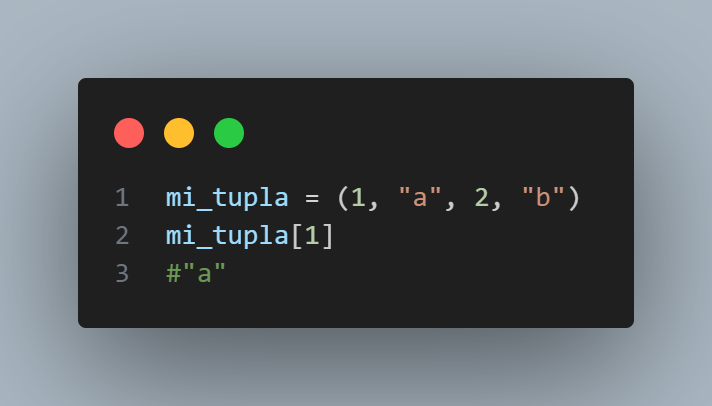
\includegraphics{Imagenes/listas16.png}
        }
      \end{figure}
    
    \item Datos inmutables: Como dije anteriormente los datos no se pueden cambiar por lo que si seleccionamos un elemento y lo tratamos de igualar a otro nos tirara un error.
    \begin{figure}[h]
        \centering
        \scalebox{0.35}{
        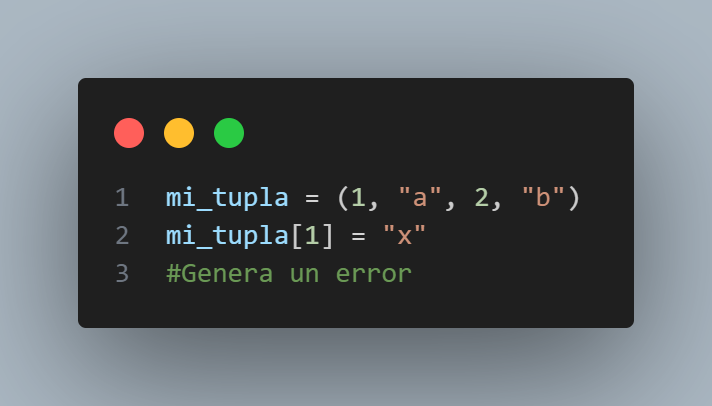
\includegraphics{Imagenes/listas17.png}
        }
      \end{figure}
    
    \item Largo de una tupla: Para saber el largo de la tupla tenemos que utilizar la función ``len(tupla)''.
    \begin{figure}[h]
        \centering
        \scalebox{0.35}{
        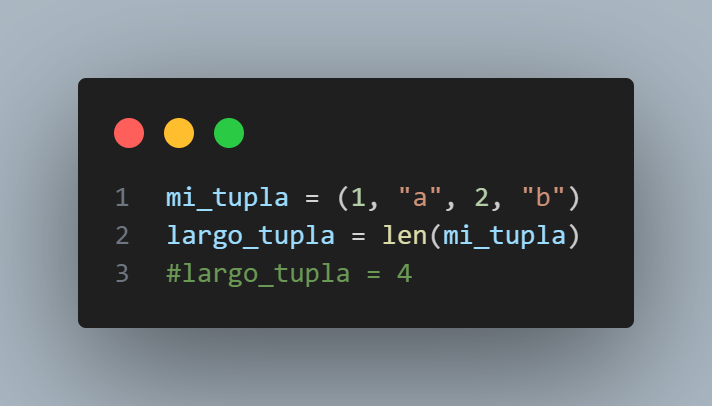
\includegraphics{Imagenes/listas18.png}
        }
      \end{figure}
    
      \newpage
    \item Rebanado (slicing): Esta propiedad sirve para seleccionar una porción de la tupla creando una nueva con estos datos y para esto necesitamos utilizar el operador de rebanado ``[:]''.
    \begin{figure}[h]
        \centering
        \scalebox{0.35}{
        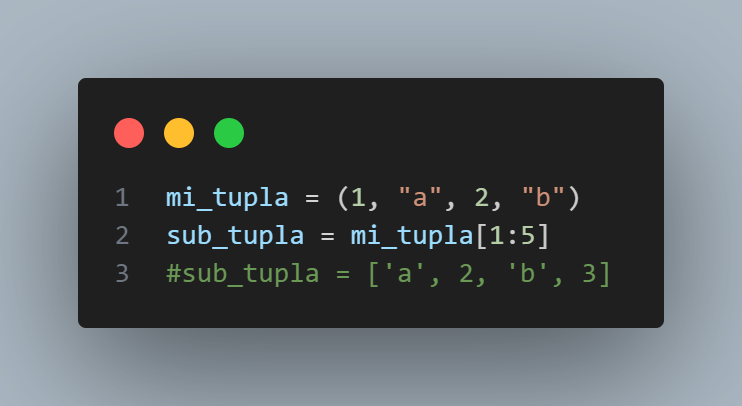
\includegraphics{Imagenes/listas19.png}
        }
      \end{figure}
    
    \item Concatenación de tuplas: Del mismo modo que en las listas para concatenar las tuplas se necesita del operador de concatenación ``+''.
    \begin{figure}[h]
        \centering
        \scalebox{0.35}{
        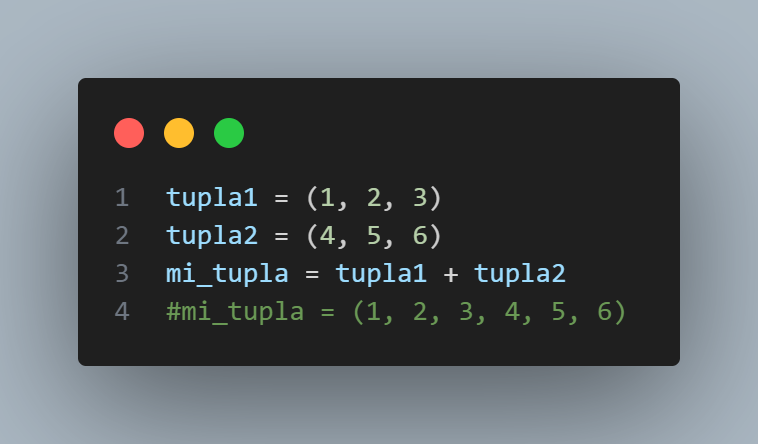
\includegraphics{Imagenes/listas20.png}
        }
      \end{figure}
    
    \item Asignación de múltiple: Este quiere decir que en una sola línea de código se puede asignar a distintas variables los elementos de la tupla. 
    \begin{figure}[h]
        \centering
        \scalebox{0.35}{
        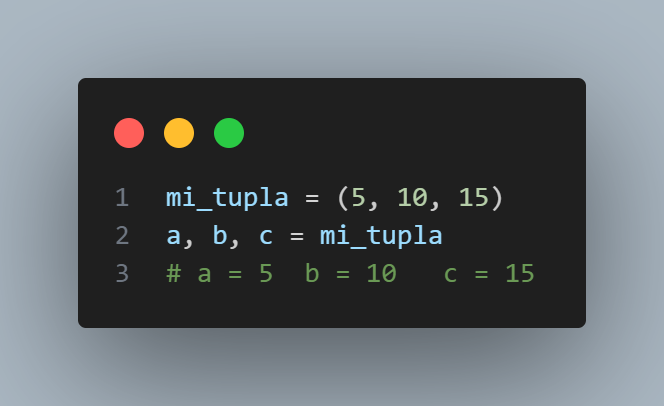
\includegraphics{Imagenes/listas21.png}
        }
      \end{figure}

\end{itemize}

\subsection{Diccionarios y métodos de acceso}
Los diccionarios en vez de las tuplas y listas contienen pares de datos que se identifican como clave-valor cada clave dentro del diccionario tiene un único valor, esto sirve para organizar todo de mejor manera y acceder a los valores de una forma mas rápida como por ejemplo:

\begin{itemize}
    \item Creación de diccionarios: Primero que nada para crear un diccionario necesitamos utilizar llaves ``{}'' y dentro separando clave-valor por ``:'' y cada par por ``,''.
    \begin{figure}[h]
        \centering
        \scalebox{0.35}{
        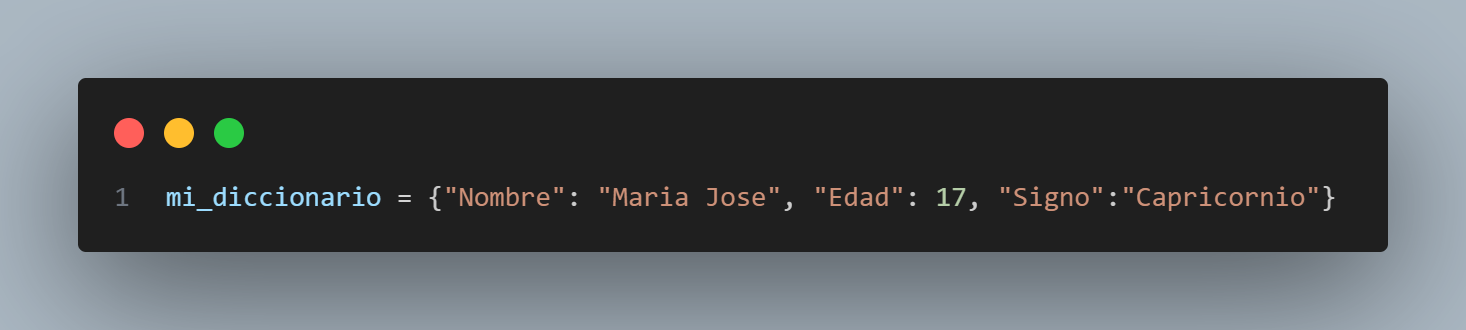
\includegraphics{Imagenes/listas22.png}
        }
      \end{figure}
    
    \item Acceso al valor: Esta vez al igual que en las anteriores se ocupan corchetes ``[clave]'' pero en vez de poner un índice esta vez se pone la clave para obtener su respectivo valor.
    \begin{figure}[h]
        \centering
        \scalebox{0.35}{
        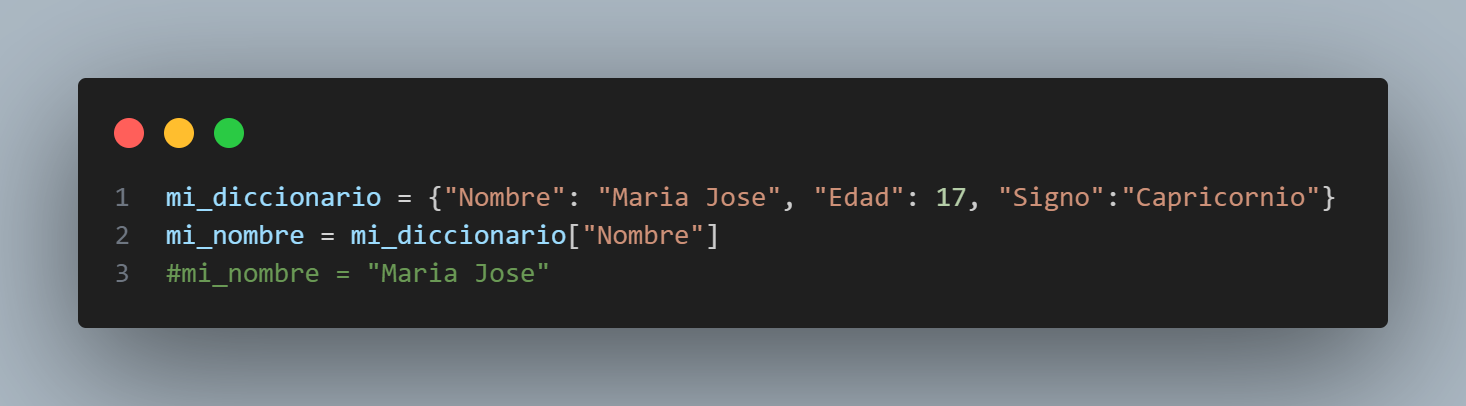
\includegraphics{Imagenes/listas23.png}
        }
      \end{figure}
    
    \item Modificación del valor: Para modificar un valor solo necesitamos seleccionar su clave e igualarlo al nuevo valor que queremos que obtenga.
    \begin{figure}[h]
        \centering
        \scalebox{0.35}{
        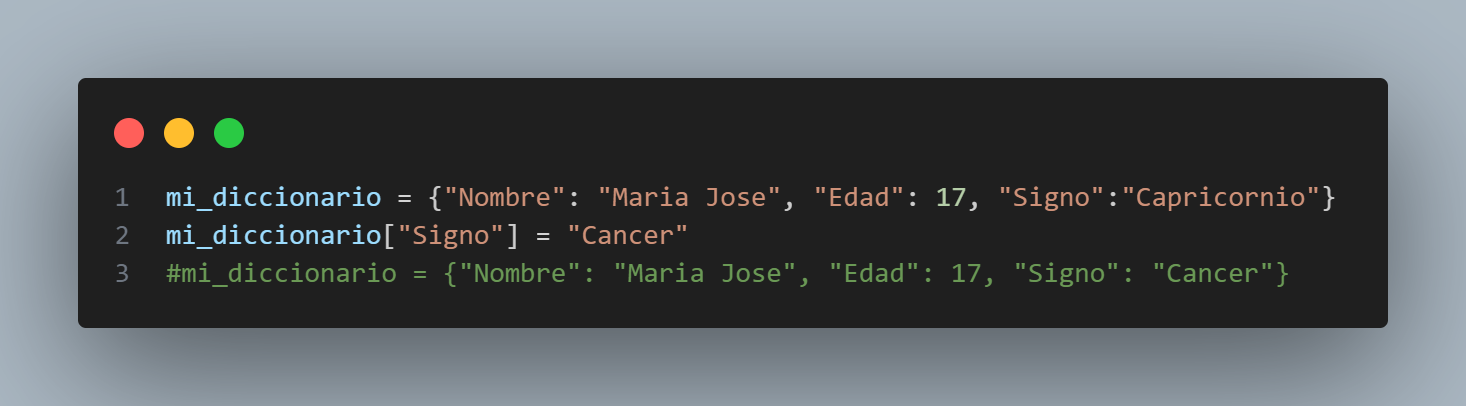
\includegraphics{Imagenes/listas24.png}
        }
      \end{figure}
    
    \item Agregar pares: Si queremos agregar nuevos pares de clave-valor solo necesitamos seleccionar una nueva clave del diccionario e igualarlo a un nuevo valor.
    \begin{figure}[h]
        \centering
        \scalebox{0.30}{
        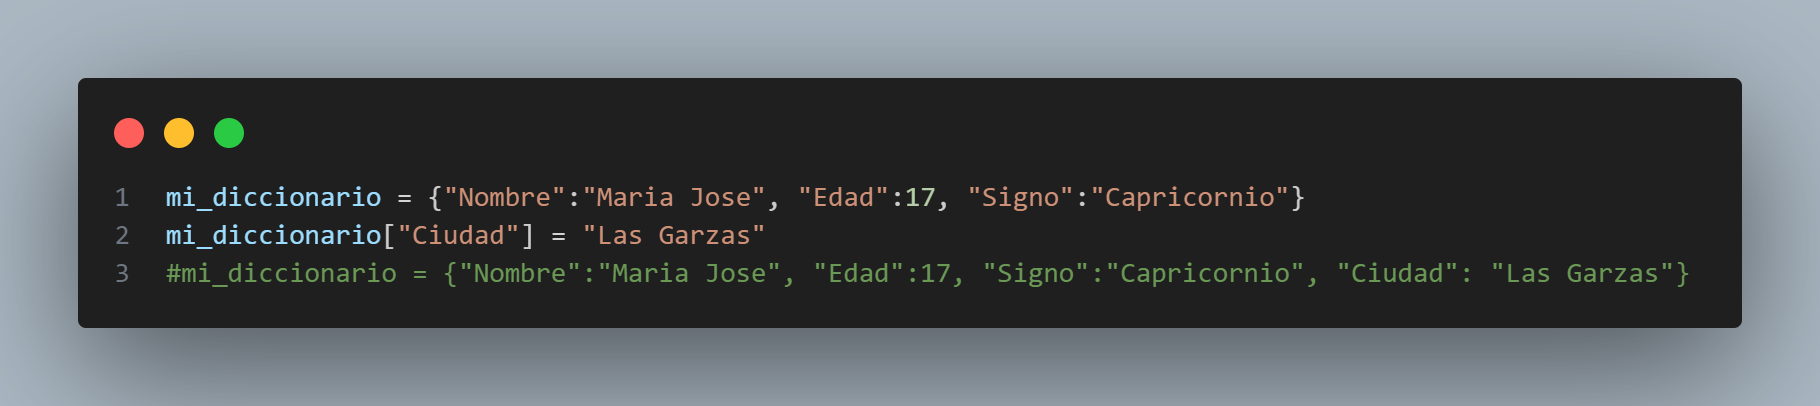
\includegraphics{Imagenes/listas25.png}
        }
      \end{figure}
    
    \item Eliminación de pares: Cuando queramos eliminar un par que este en el diccionario solo debemos utilizar la declaración ``del'' y especificar la clave.
    \begin{figure}[h]
        \centering
        \scalebox{0.35}{
        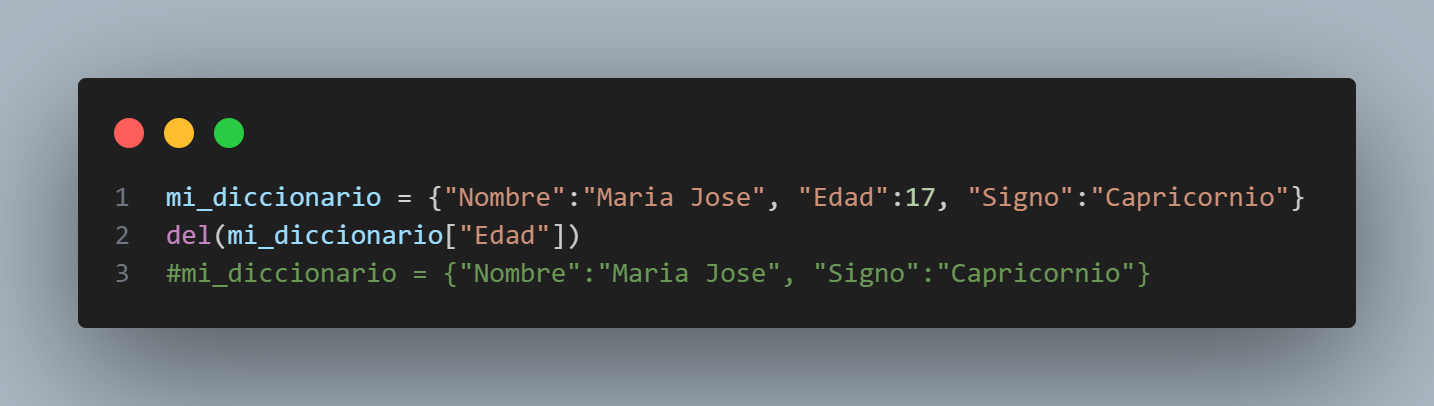
\includegraphics{Imagenes/listas26.png}
        }
      \end{figure}
    
    \item Verificación de existencia de clave: Para verificar si una clave en específico existe dentro de un diccionario podemos utilizar el operador ``in''.
    \begin{figure}[h]
        \centering
        \scalebox{0.35}{
        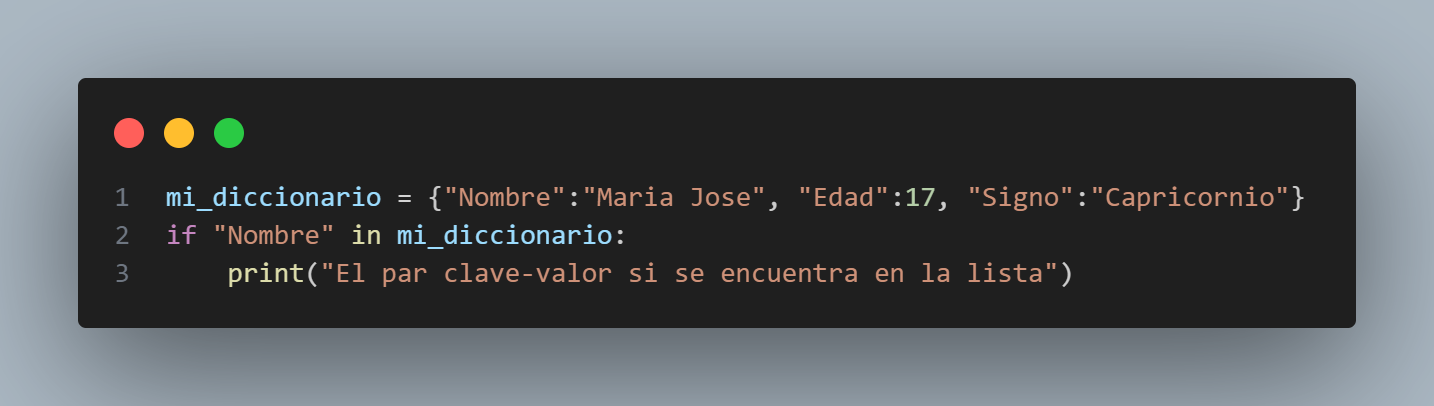
\includegraphics{Imagenes/listas27.png}
        }
      \end{figure}
    
    \item  Obtener clave-valor: Para obtener o todas las claves o todos los valores de un diccionario podemos utilizar los métodos ``.keys()'' o ``.values()'' respectivamente, pero si queremos obtener el par de elementos utilizaremos el método ``.items()''.
    \newpage
    \begin{figure}[h]
        \centering
        \scalebox{0.35}{
        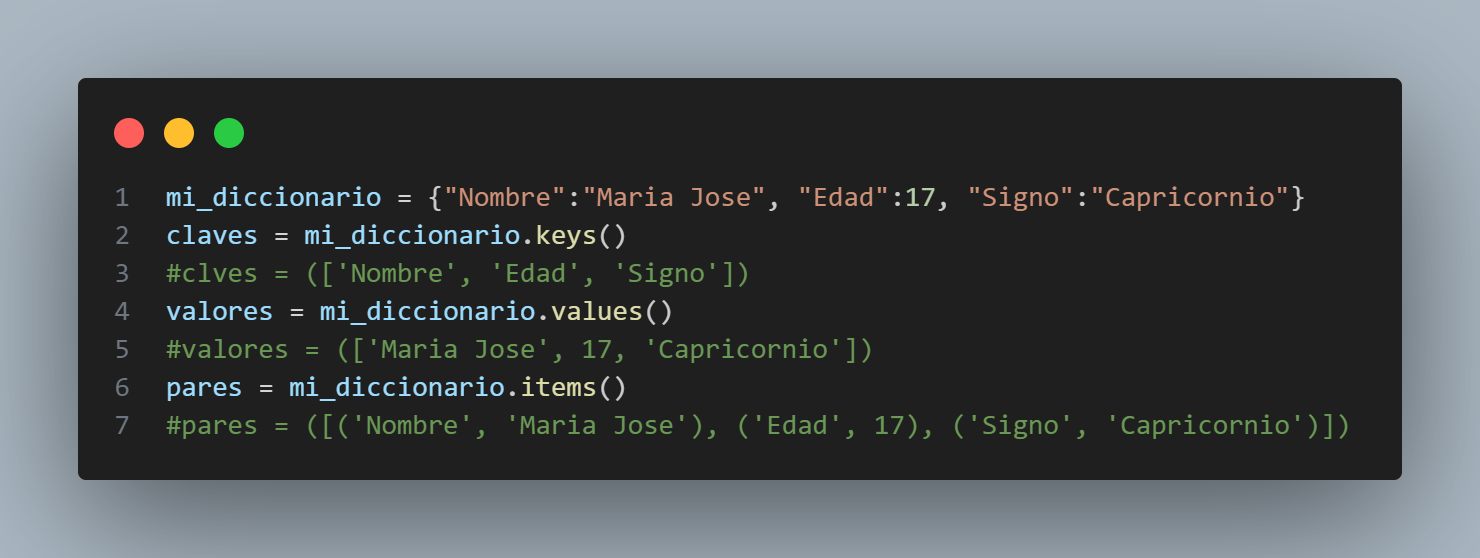
\includegraphics{Imagenes/listas28.png}
        }
      \end{figure}

\end{itemize}